%%%%%%%%%%%%%%%%%%%%%%%%%%%%%%%%%%%%%%
%%%%%%%%%%%%%%%%%%%%%%%%%%%%%%%%%%%%%%
% Do not edit the TeX file your work
% will be overwritten.  Edit the RnW
% file instead.
%%%%%%%%%%%%%%%%%%%%%%%%%%%%%%%%%%%%%%
%%%%%%%%%%%%%%%%%%%%%%%%%%%%%%%%%%%%%%






\newcommand{\ElectionData}{

\begin{knitrout}
\definecolor{shadecolor}{rgb}{0.969, 0.969, 0.969}\color{fgcolor}

{\centering 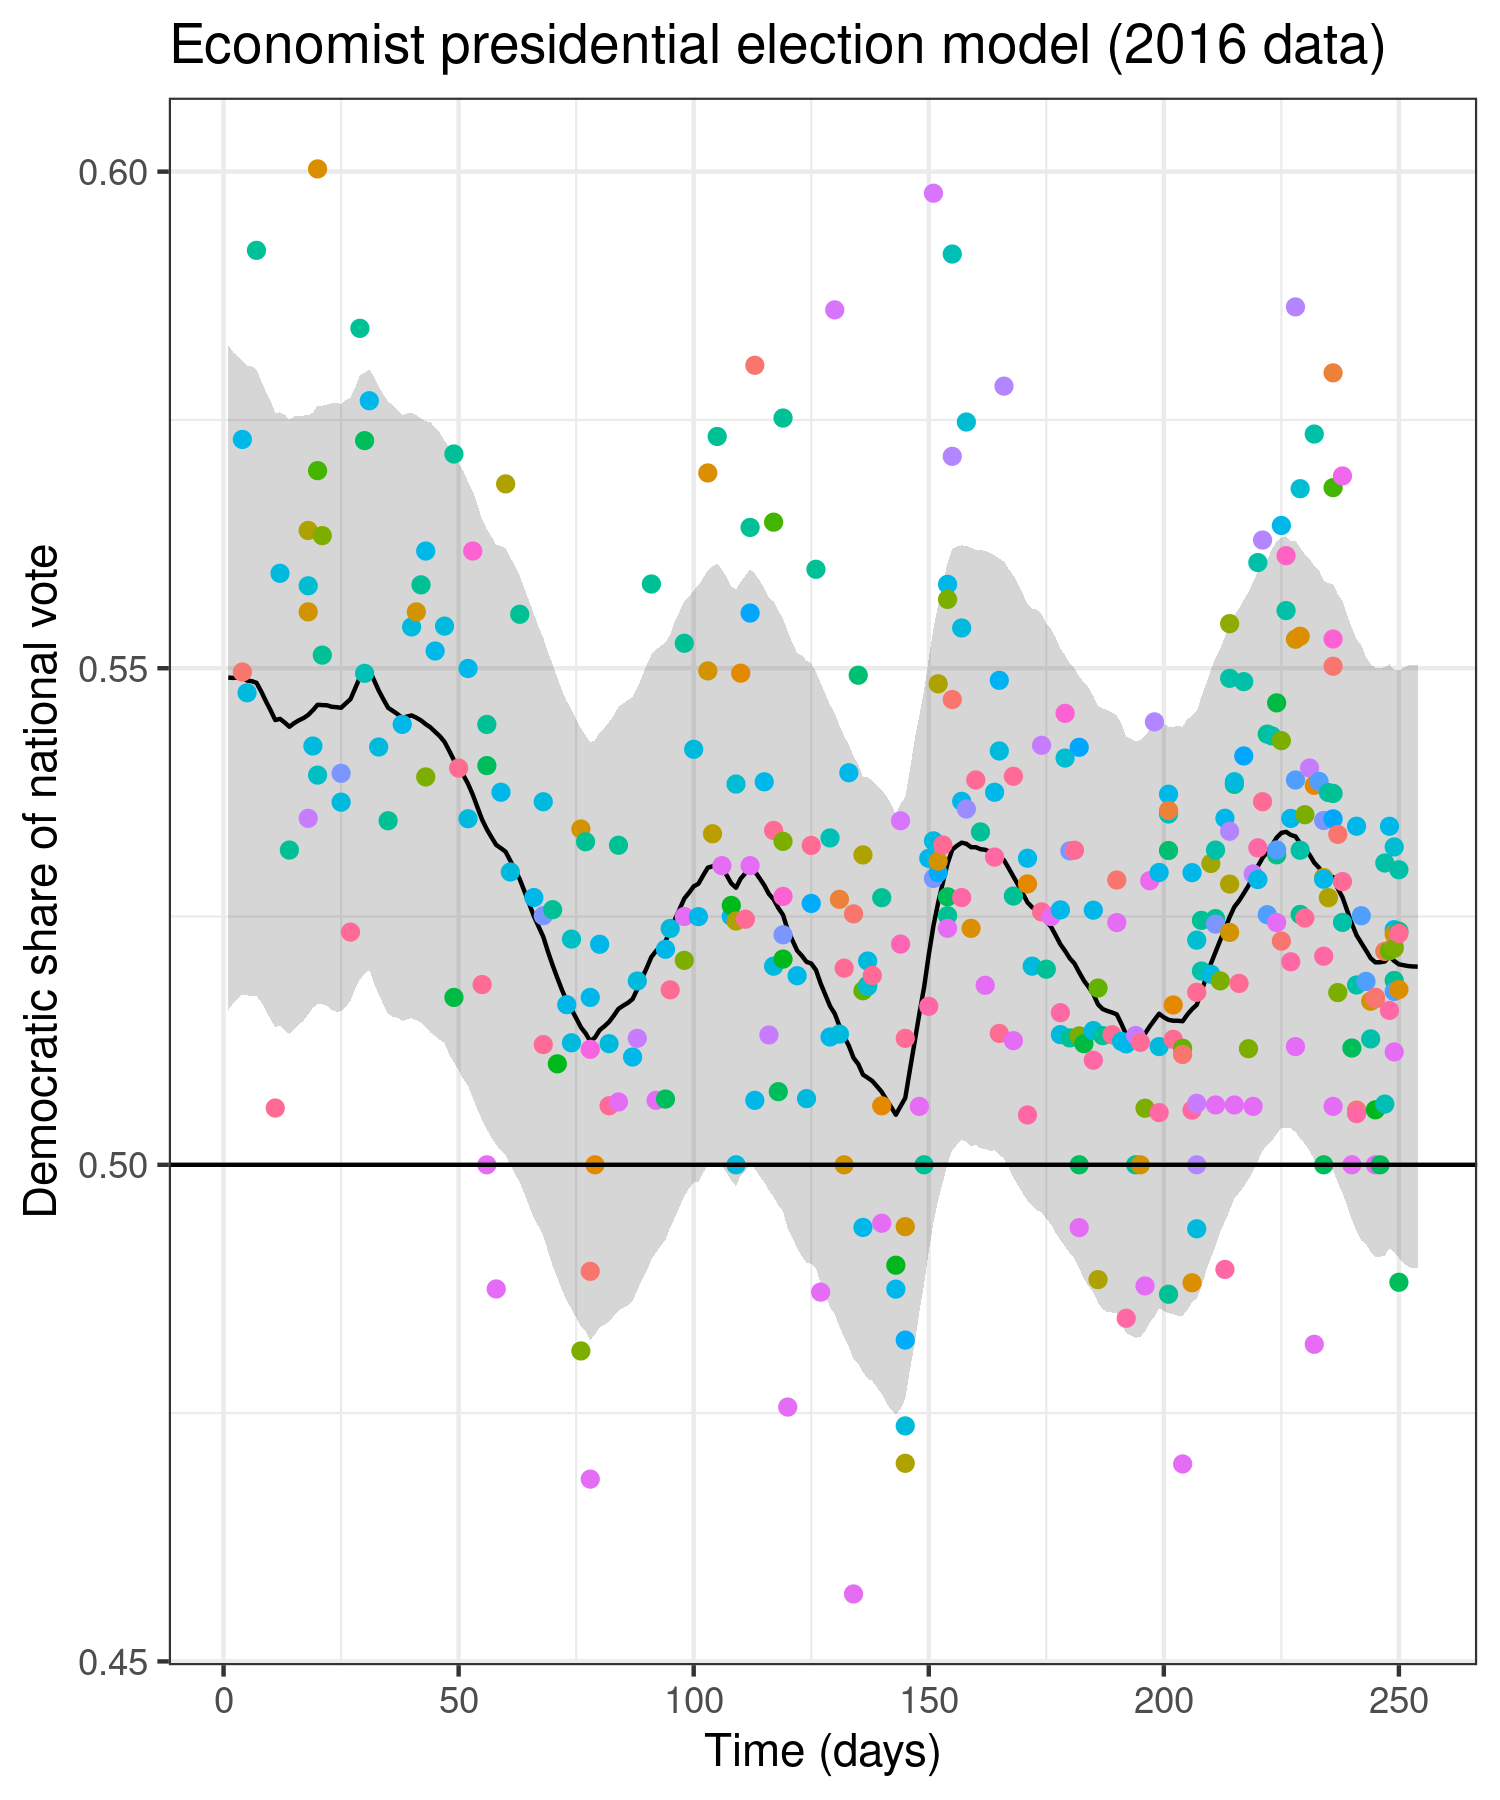
\includegraphics[width=0.980\linewidth,height=1.176\linewidth]{figure/election_data-1} 

}



\end{knitrout}
}


\newcommand{\ElectionResultsGlobal}{

\begin{knitrout}
\definecolor{shadecolor}{rgb}{0.969, 0.969, 0.969}\color{fgcolor}

{\centering 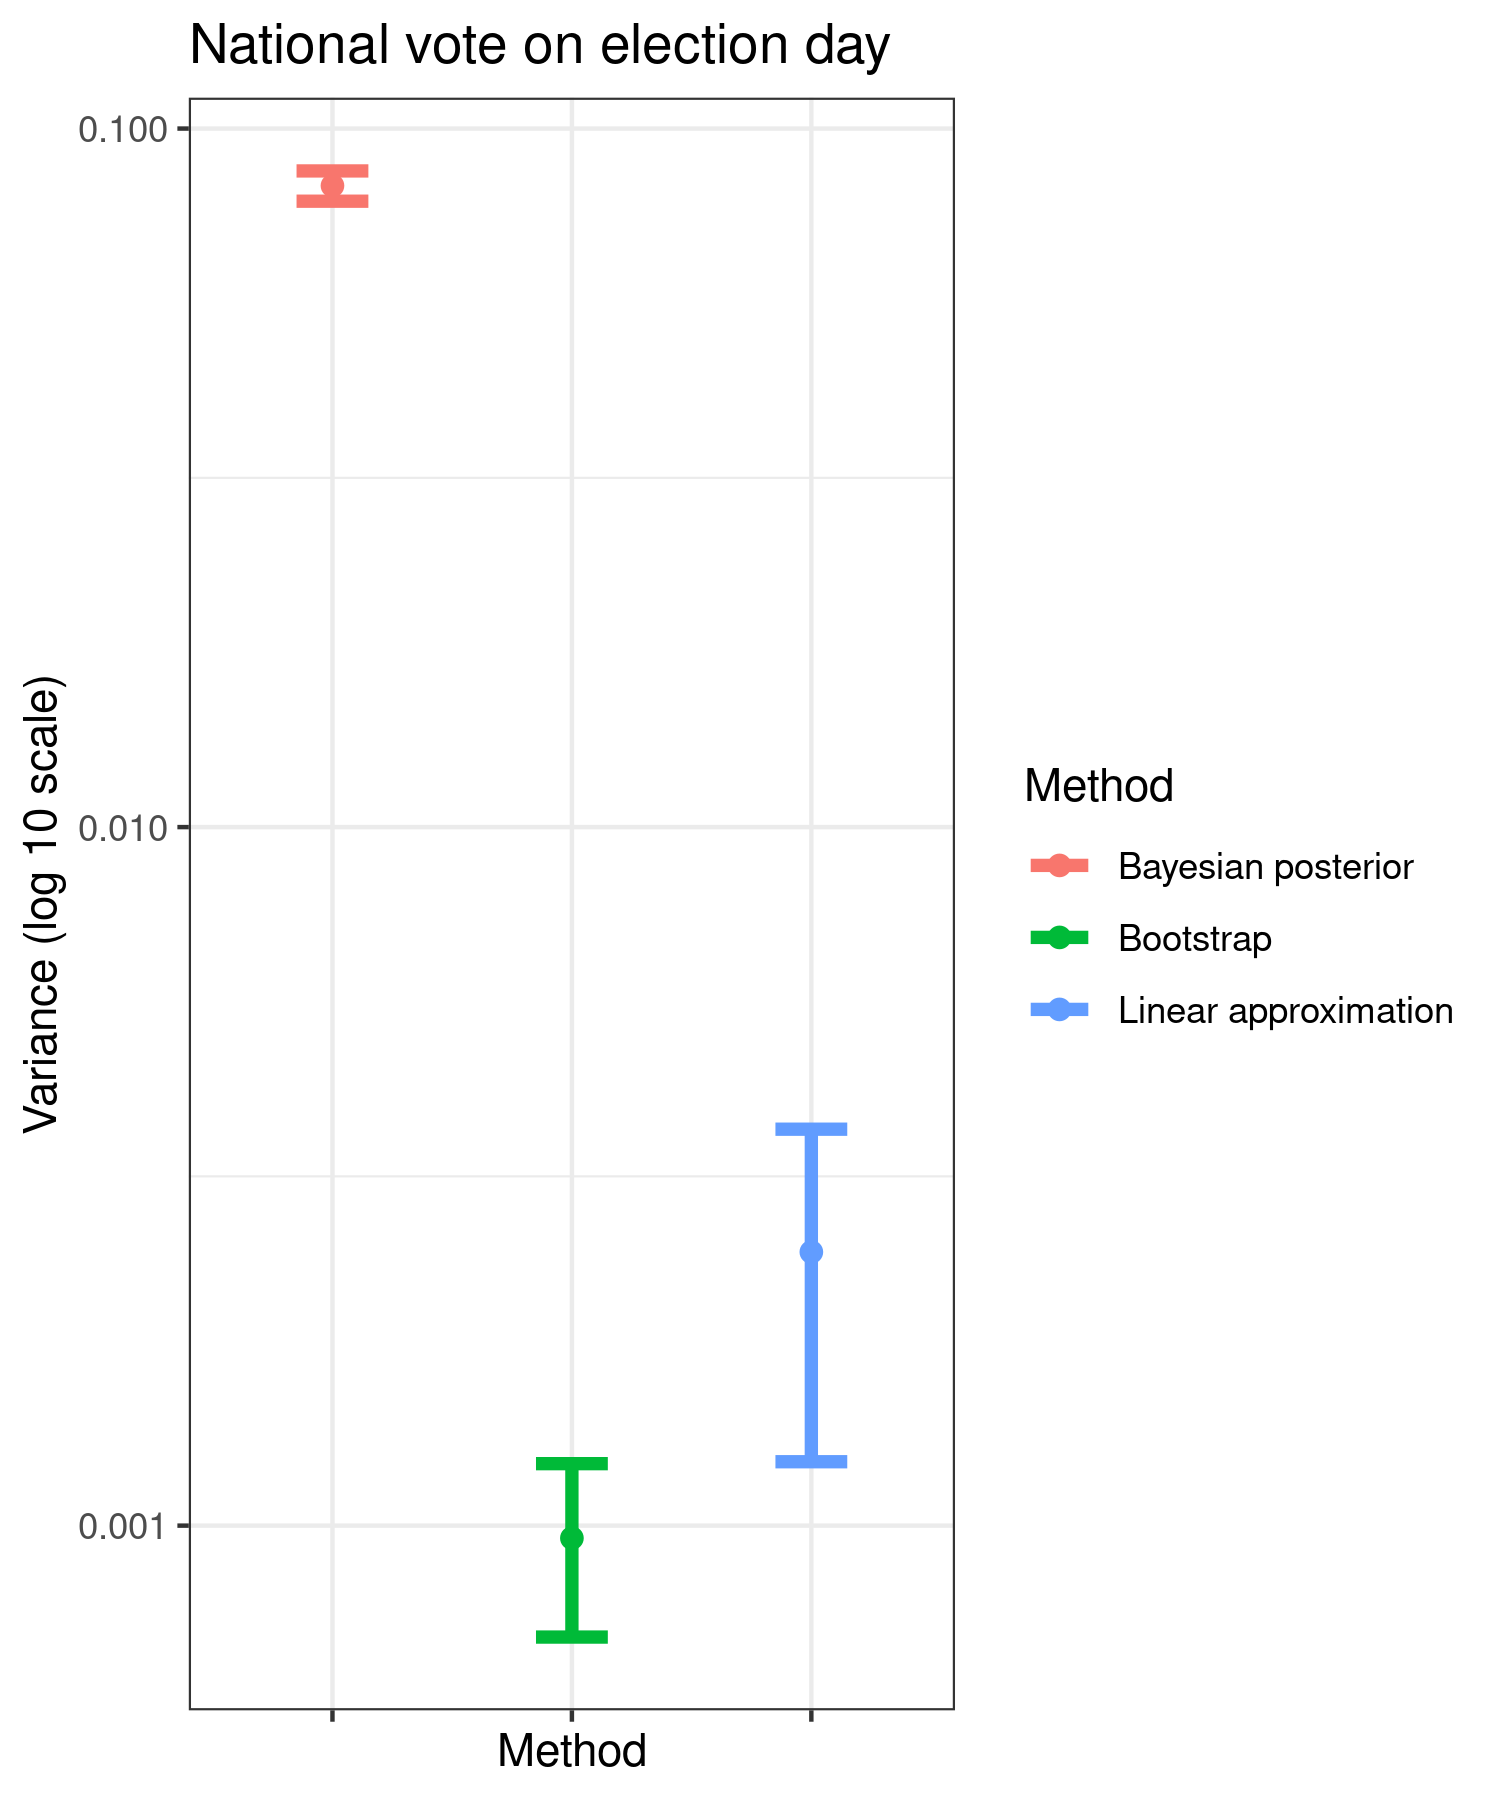
\includegraphics[width=0.980\linewidth,height=1.176\linewidth]{figure/election_result-1} 

}



\end{knitrout}
}




\newcommand{\PoissonFigTen}{

\begin{knitrout}
\definecolor{shadecolor}{rgb}{0.969, 0.969, 0.969}\color{fgcolor}

{\centering 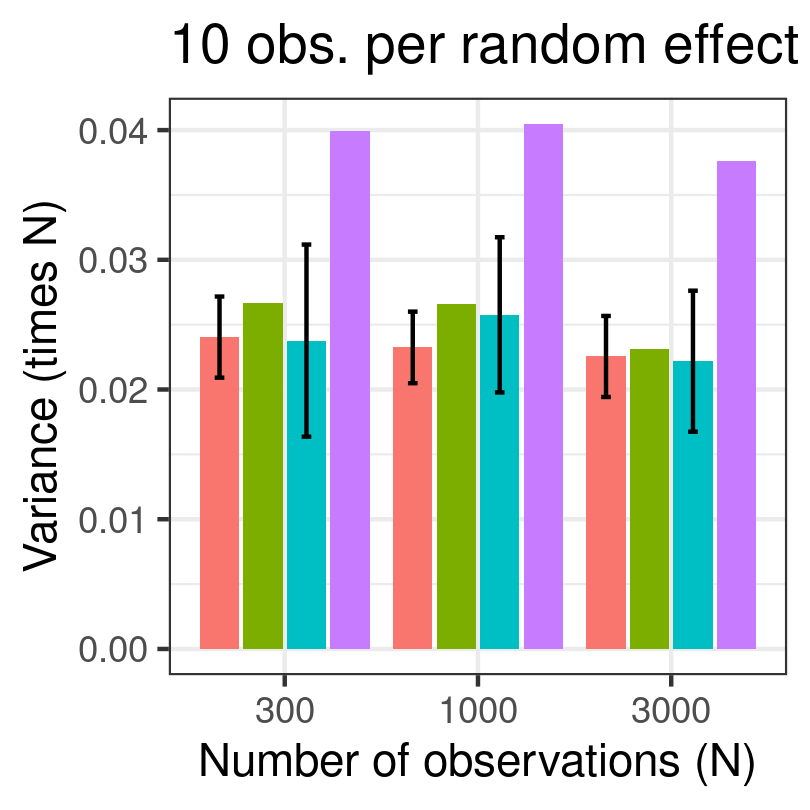
\includegraphics[width=0.980\linewidth,height=0.980\linewidth]{figure/PoissonFigTen-1} 

}



\end{knitrout}
}


\newcommand{\PoissonFigOne}{

\begin{knitrout}
\definecolor{shadecolor}{rgb}{0.969, 0.969, 0.969}\color{fgcolor}

{\centering 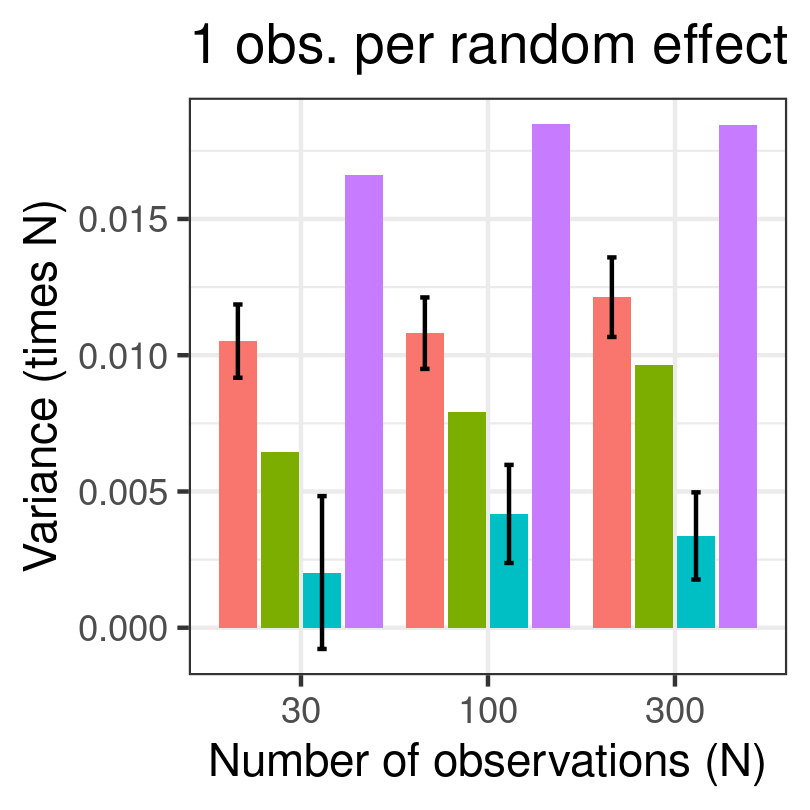
\includegraphics[width=0.980\linewidth,height=0.980\linewidth]{figure/PoissonFigOne-1} 

}



\end{knitrout}
}


\newcommand{\PoissonFigLegend}{

\begin{knitrout}
\definecolor{shadecolor}{rgb}{0.969, 0.969, 0.969}\color{fgcolor}

{\centering 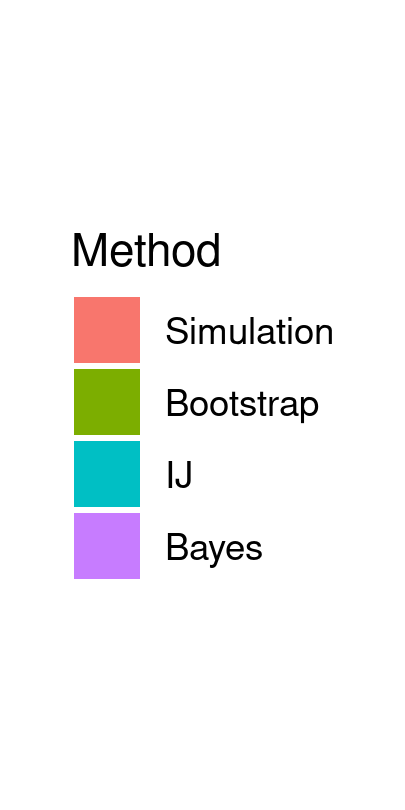
\includegraphics[width=0.980\linewidth,height=1.960\linewidth]{figure/PoissonFigLegend-1} 

}



\end{knitrout}
}



\newcommand{\ARMRelFig}{

\begin{knitrout}
\definecolor{shadecolor}{rgb}{0.969, 0.969, 0.969}\color{fgcolor}

{\centering 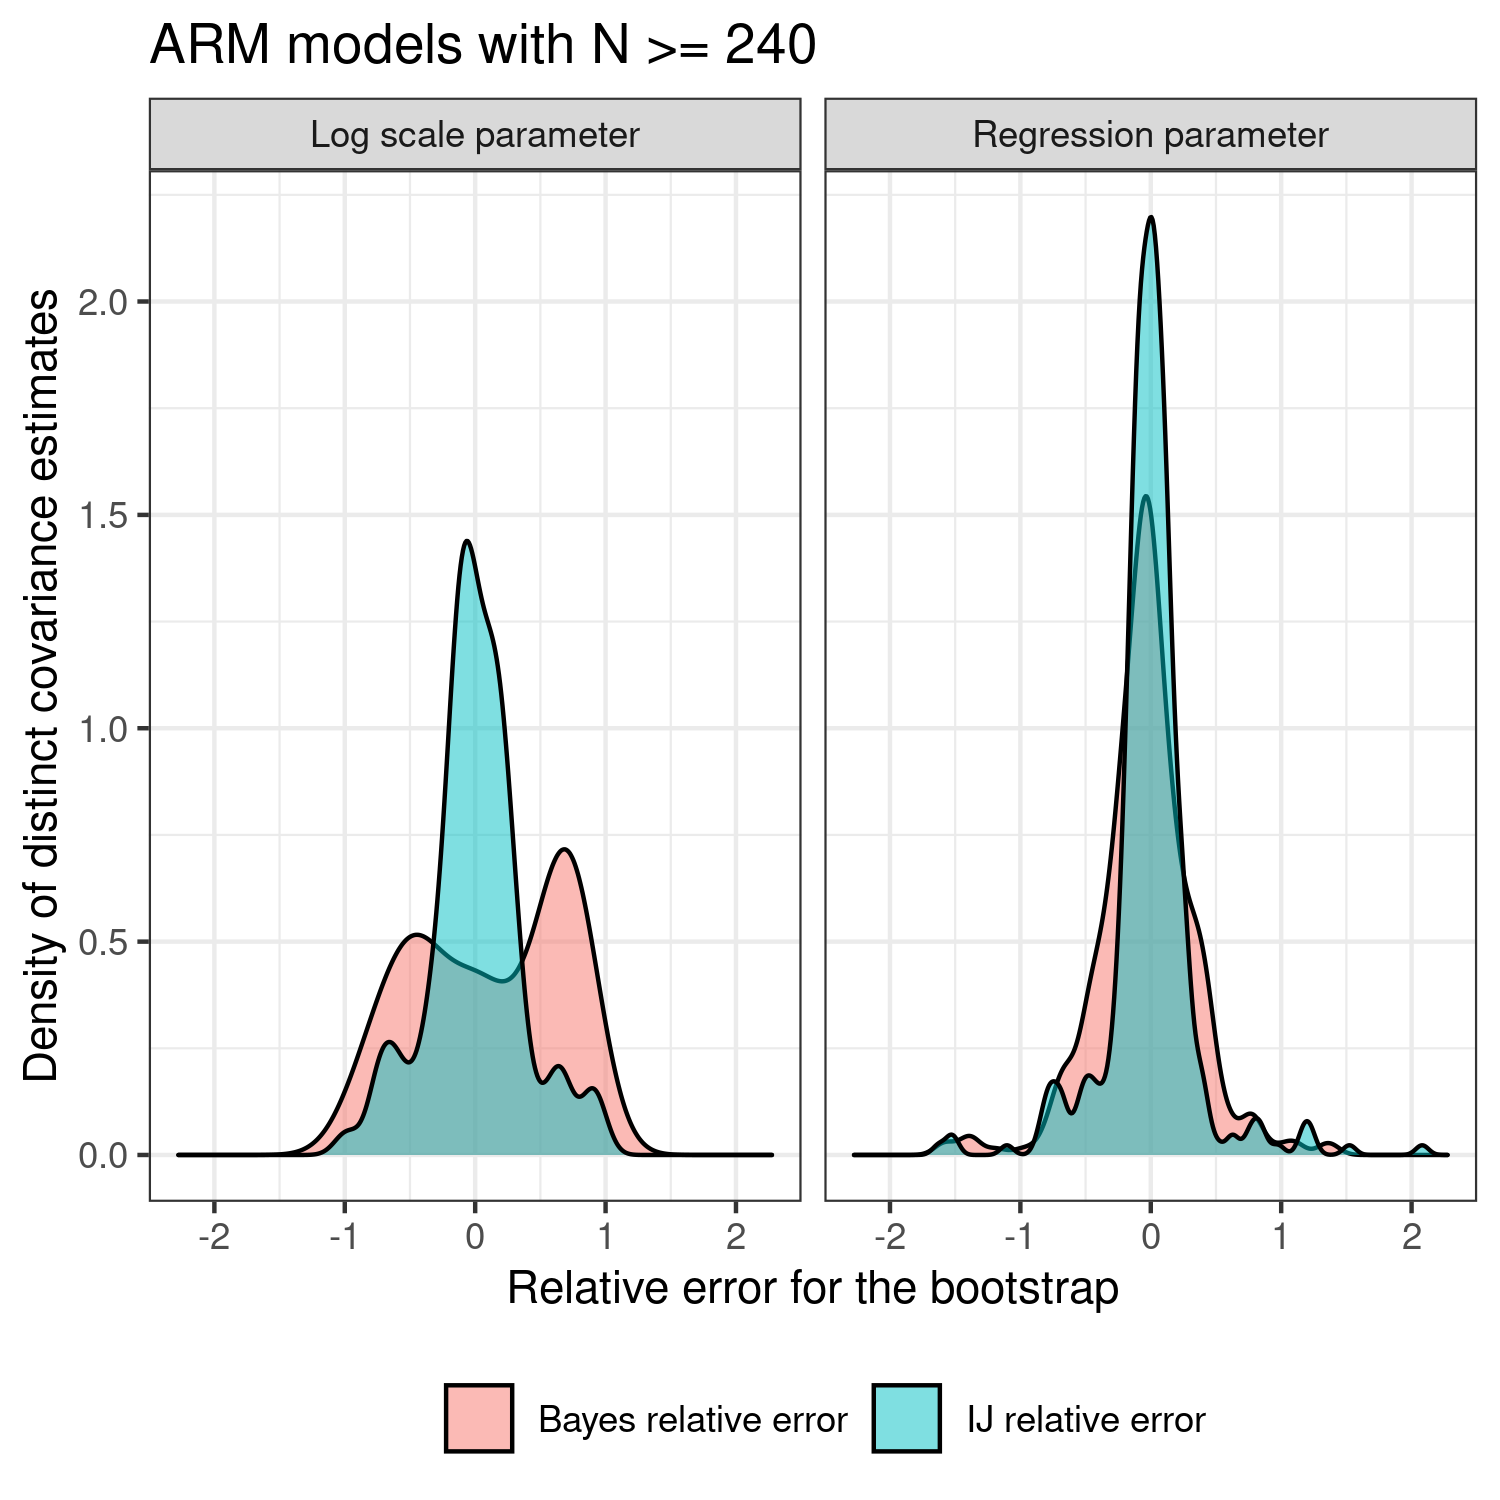
\includegraphics[width=0.980\linewidth,height=0.980\linewidth]{figure/normerr_graph-1} 

}



\end{knitrout}
}


\newcommand{\ARMZFig}{

\begin{knitrout}
\definecolor{shadecolor}{rgb}{0.969, 0.969, 0.969}\color{fgcolor}

{\centering 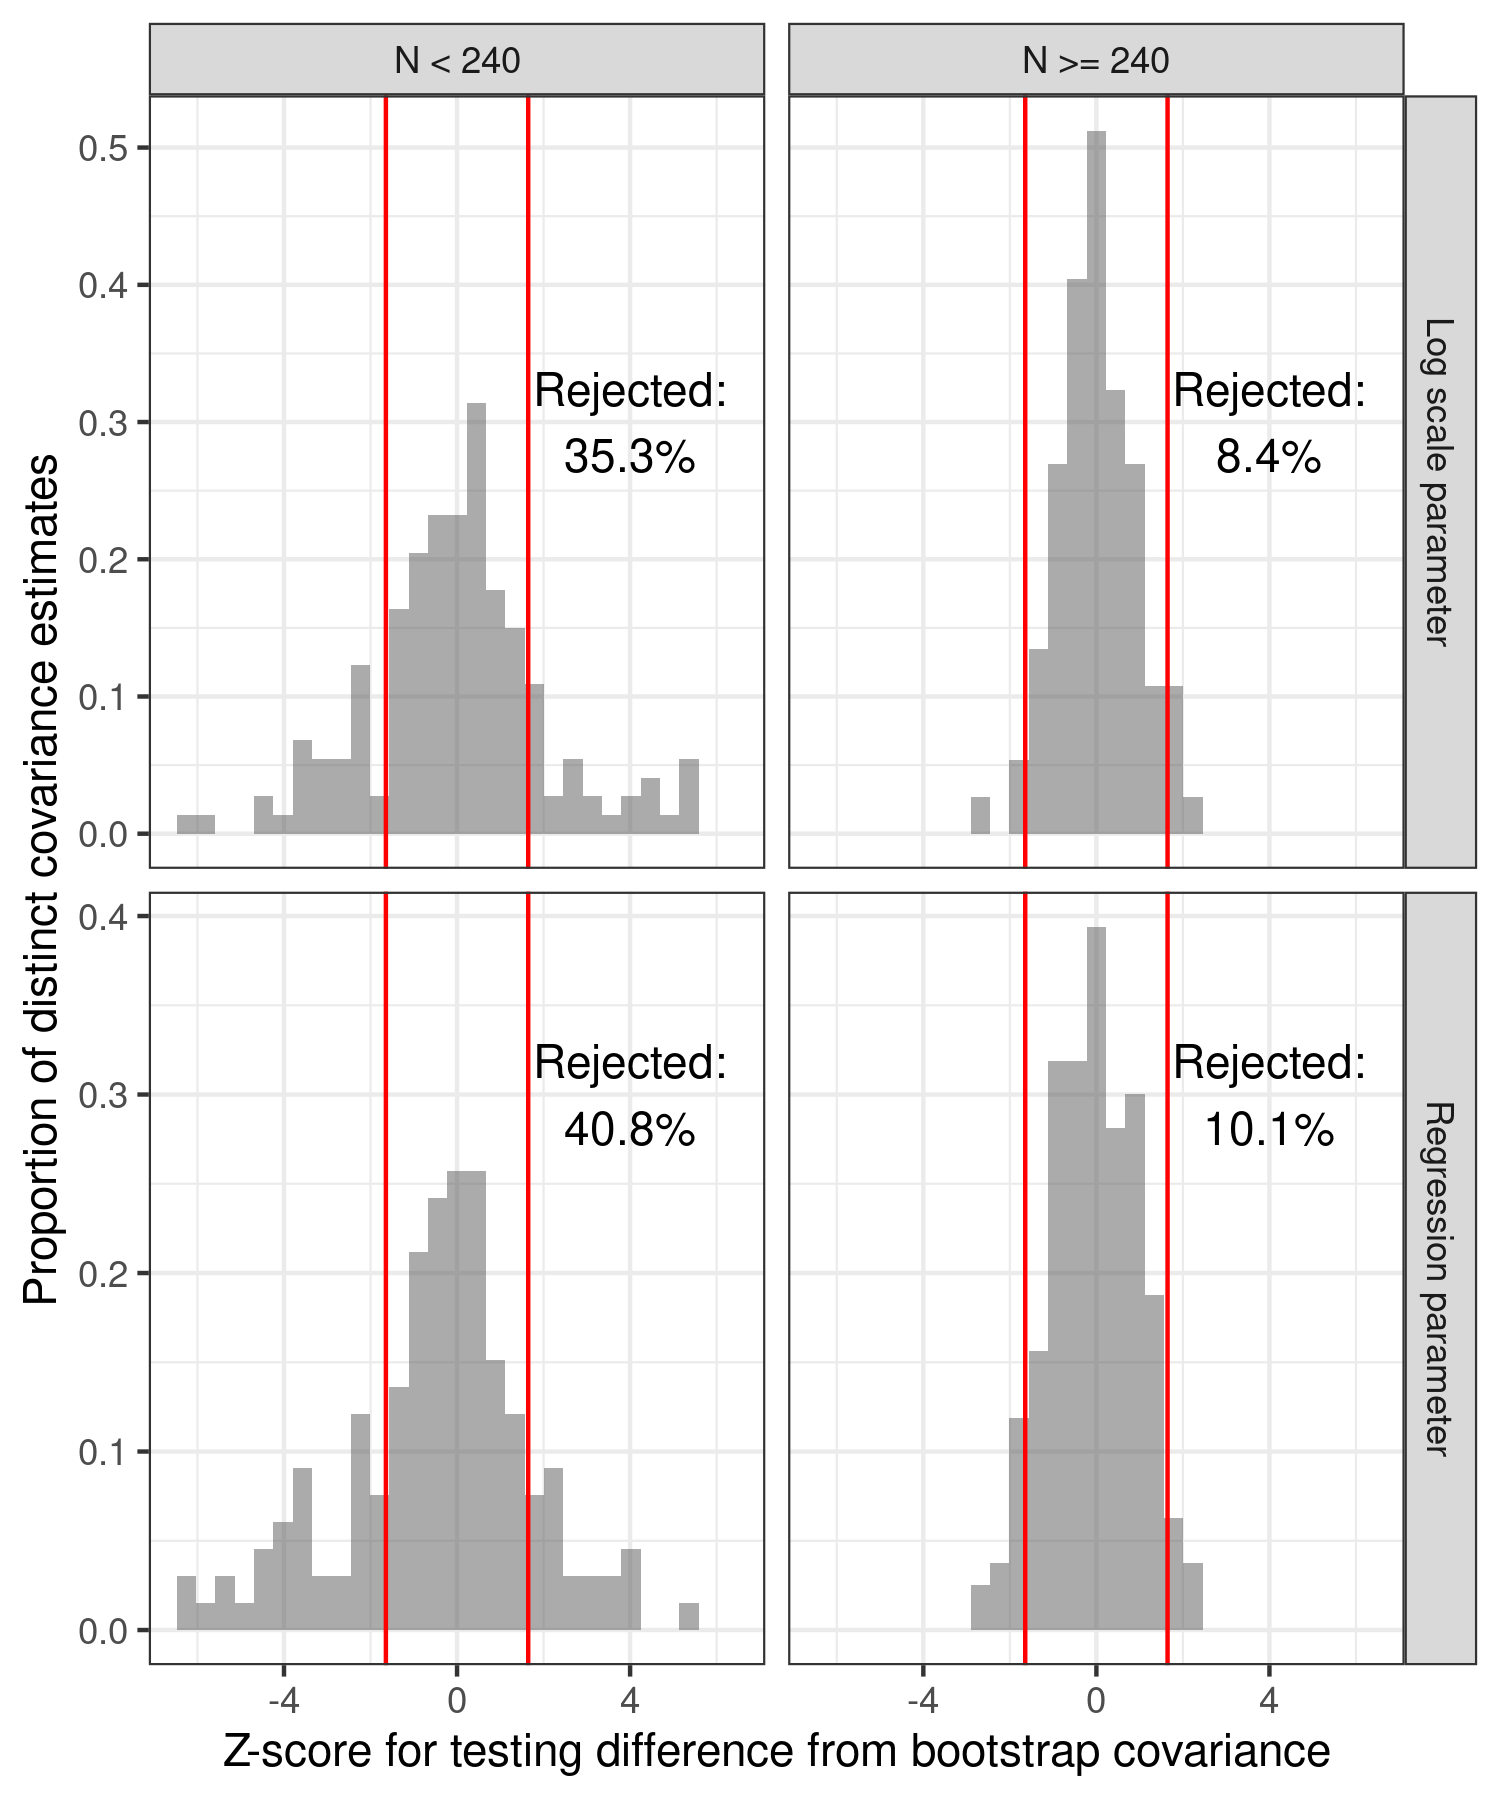
\includegraphics[width=0.980\linewidth,height=1.176\linewidth]{figure/relerr_graph-1} 

}



\end{knitrout}
}
